% !TEX program = pdflatex
% !BIB program = biber

% !TEX root = main.tex
\documentclass[10pt, a4paper]{article}
% \documentclass[12pt, a4paper, oneside]{memoir}
% \chapterstyle{veelo}

%% Sets page size and margins
\usepackage[a4paper,top=3cm,bottom=2cm,left=3cm,right=3cm,marginparwidth=1.75cm]{geometry}
%\usepackage[left=2cm,top=2cm,bottom=2cm,bindingoffset=1cm]{geometry}

\usepackage[utf8x]{inputenc}
\usepackage{graphicx}
\usepackage{float}
\usepackage{imakeidx}
\usepackage{amsmath}
\usepackage[colorlinks=true, allcolors=blue]{hyperref}
\usepackage{graphicx}
\usepackage{float}
\usepackage{imakeidx}
\usepackage{amsmath}
\usepackage{url}
\usepackage[export]{adjustbox}
\usepackage{subcaption}

%% Useful packages
\usepackage[colorinlistoftodos]{todonotes}
\usepackage[T1]{fontenc}

%% Language and font encodings
\usepackage[english]{babel}

%% Define a few colours to be used throughout the document
\usepackage{tikz,xcolor}
\definecolor{TextColor}{HTML}{000000}
\definecolor{SideColorDark}{HTML}{000000}
\definecolor{MainColor}{HTML}{0000FF}
\definecolor{OppositeColor}{HTML}{FF0000}
\definecolor{HighlightColor}{HTML}{FFFF00}


%% Code block style
%  Load the \ttfamily font
\usepackage[T1]{fontenc}
\usepackage[scaled]{beramono}

%  Format code blocks
\usepackage{listings}
%  Change caption name
\renewcommand*{\lstlistingname}{Code block}
\captionsetup[lstlisting]{margin=0cm,format=hang,font=small,format=plain,labelfont={bf,up},textfont={it}}
%  Style
\lstset{
  showstringspaces=false,
  formfeed=\newpage,
  commentstyle=\itshape,
  backgroundcolor=\color{gray!5},
  breakatwhitespace=false,         % sets if automatic breaks should only happen at whitespace
  breaklines=true,                 % sets automatic line breaking
  captionpos=b,                    % sets the caption-position to bottom
  commentstyle=\color{gray},    % comment style
  escapeinside={\%*}{*)},          % if you want to add LaTeX within your code
  keepspaces=true,
  numbersep=2mm,                   % how far the line-numbers are from the code
  showspaces=false,
  showstringspaces=false,
  showtabs=false,
  stepnumber=1, numberfirstline=false,
  basicstyle=\linespread{1}\footnotesize\ttfamily,
  keywordstyle=\bfseries\color{MainColor},
  stringstyle=\itshape\color{OppositeColor},
  numberstyle=\footnotesize\ttfamily\color{gray},
  numbers=left,xleftmargin=4mm,framexleftmargin=0mm,xrightmargin=0mm,
  frame=top,frame=bottom,
}

\title{CS414 Practical 2}
\author{Leandra Geldenhuys\\17534666\\\\Daniel Robinson\\18361137}

\begin{document}
% \maketitle
    \begin{titlepage}
        \begin{center}
            \vspace*{1cm}
            
            \huge
            \textbf{CS414 Practical 2\\Preliminary Design Review}
            
            \vspace{1.5cm}
            
            \large
            Leandra Geldenhuys\\
            17534666\\
            \vspace{2.5cm}
            Heinrich\\
            17..\\
            \vspace{2.5cm}
            Aanchal Katiyar\\
            18613435\\
            \vspace{2.5cm}
            Daniel Robinson\\
            18361137\\
            \vspace{4.5cm}
            
            \large
            Date: 7 February 2017
            
        \end{center}
\end{titlepage}

\tableofcontents
\listoffigures
\listoftables

\newpage

% \begin{abstract}
% Your abstract.
% \end{abstract}

\section{Systems Overview}

In this section the mission objectives and requirements are specified.

\subsection{Mission Objectives}
In order to be deemed successful the CanSat system needs to complete the following missions:

\begin{itemize}
    \item The CanSat will be launched from approximately 1000m by a rocket.  The CanSat will then be ejected from the rocket.
    \item Measurements of air pressure and temperature will be taken during decent.
    \item These measurements will be transmitted at least once every second to the ground station.
    \item On the ground station the received data will be analysed.
\end{itemize}

\section{System Level Requirements}
The system has certain constraints and requirements it must adhere to:
\begin{itemize}
    \item The total mass should be between 490 and 510 grams.
    \item All components (except parachute, antenna and GPS) should fit inside a can with a height of 115 mm and 66 mm diameter.
    \item The container should fit inside a cylindrical envelope with a height of 310 mm and 66 mm diameter.
    \item System should use a passive control system, with a controlled decent speed between 8 and 11 m/s.
    \item All electronics should be enclosed, shielded from the environment and hard mounted.
    \item The system should be able to survive 15 Gs acceleration.
    \item The system should be powered by alkaline batteries which should be easily accessible.
    \item All materials used must be safe for personnel, equipment and the environment. 
\end{itemize}

\subsection{Architecture}

\newpage

\section{Sensor Subsystem Design}
In this section the sensors of the system is designed.
\subsection{Subsystem Requirements}
The sensors needs to adhere to certain requirements:
\begin{itemize}
    \item System needs to be able to read air pressure, temperature and determine its dynamic state.
    \item The system needs to wake up when CanSat is launched from the rocket.
    \item All sensors need to be able to withstand extreme weather conditions and up to 15Gs.
\end{itemize}
\subsection{CanSat Sensor System}
\subsubsection{Launch Recognition}
In order for the system to recognize when it has been launched from the rocket, a type of switch needs to be designed.   The switch will turn on the power system and enable the CanSat to start reading from the sensors and transmitting to the ground.
\subsubsection{Attitude and Dynamic State}
To measure the attitude of the CanSat, a three axes sensor is needed that provide attitude information, including roll, pitch and yaw.  The dynamic state can be determined using a gyroscope, accelerometer and magnetometer. 
\subsubsection{Air Pressure and Temperature}
The air pressure and temperature needs to be taken during the CanSat's decent.  
\subsection{Trade Studies and Selections}
\subsubsection{Launch Recognition}
Possible designs include contact switches, magnetic switches and optical sensors.  Keeping the extreme conditions the switch circuit will have to endure in mind, a strong, durable contact switch is the best option.  The switch chosen for this design is the B5112 Normally Closed Pushbutton Switch from Control Products Inc. (seen in Figure~\ref{fig:p}). These switches are covered with thermoplastic and can withstand temperatures between 10 and 105 degrees Celsius.  According the Control Products Inc, their switches perform well "under the wettest, and harshest environmental conditions" which makes it ideal for this application.  It measures 20.57x40.89x9.52mm.
\subsubsection{Attitude and Dynamic State}
There are various different models of gyroscopes, accelerometers and magnetometers available on the market,  For this application, size and weight is a huge factor in the selection process.  For this reason an 'all in one' solution was chosen.  The IvenSense MPU-9250 (seen in Figure~\ref{fig:att}) is a 9-axis MotionTracking device which consists of a gyroscope, accelerometer and magnetometer.  It can also connect to third-party sensors using $I^2C$ communication.  The sensor is very small, 3x3x1 mm and can withstand up to 10 000 Gs.
\subsubsection{Air Pressure and Temperature}
Again, there are many different models of pressure and temperature sensors available on the market.  It is important that the chosen sensor can be used for this application.  The Altimeter Module MS5607 (seen in Figure~\ref{fig:pres}) from Parallax reads pressure and temperature, is small (2.16x2.03mm) and is used for high altitude balloons and altitude hold for UAVs, which makes it ideal.  This sensor can also communicate with the IvenSense sensor via $I^2C$.

\begin{figure}[H]
\begin{subfigure}{0.5\textwidth}
\includegraphics[scale=0.3]{3.png}
\caption{Pushbutton Switch.\\
Reproduced from \cite{cpi}.}
\label{fig:p}
\end{subfigure}
\begin{subfigure}{0.5\textwidth}
\centering
\includegraphics[scale=0.1]{2.png}
\caption{IvenSense MPU-9250.\\
Reproduced from\cite{iven}.}
\label{fig:att}
\end{subfigure}
\begin{subfigure}{0.5\textwidth}
\centering
\includegraphics[scale=0.3]{1.png}
\caption{Altimeter Module MS5607.\\ Reproduced from \cite{par}.}
\label{fig:pres}
\end{subfigure}
\caption{Sensors}
\label{fig:sensors}
\end{figure}

\newpage

\section{Mechanical Subsystem Design}
\subsection{Overview}
\subsection{Key Trade Issues}
\subsection{Preliminary Mass Budget}

\newpage

\section{Communication and Data Handling Subsystem Design}
\subsection{Requirements}
\begin{itemize}
    \item System needs to be able to transmit atmospheric pressure and temperature to the GCS (Ground Control Station) during descent.
    %% TODO: add footer to GCS
    \item Interfacing to external sensors.
    \item Storage is required for attitude data.
    \item Ability to progress through different flight modes.
\end{itemize}
\subsection{Communication and Data Handling System}
\subsubsection{Data Packet}

The data must be transmitted at least every second.\\

In order for the data to be transmitted successfully, it needs to be in a format acceptable by the GCS. The data will be stored in a JSON packet created using a C++ library\cite{ajson}.

Code block \ref{code:json1} shows a potential data packet.

\lstset{language=html,caption={Potential packet},label=code:json1}
\begin{lstlisting}
{
  "temperature": "11.3",
  "pressure": "99.325"
}
\end{lstlisting}

To verify the data on the GCS, we can perform a CRC-CCITT checksum on the data values\cite{crc-cal}.\\

In Code block \ref{code:crc}, a space is inserted between the values, and a checksum is returned using this library\cite{crc-lib}.

\lstset{language=html,caption={Checksum of values},label=code:crc}
\begin{lstlisting}
"11.3 99.325"  =>  "1E 18"
\end{lstlisting}

\lstset{language=html,caption={Potential packet with CRC checksum},label=code:packet_crc}
\begin{lstlisting}
{
  "temperature": "11.3",
  "pressure": "99.325",
  "crc": "1E18"
}
\end{lstlisting}

In Code block \ref{code:packet_notags}, the tag values are not necessary to send, since the values are based on position/index.


\lstset{language=html,caption={Potential packet with tags removed},label=code:packet_notags}
\begin{lstlisting}
{
  "11.3",
  "99.325",
  "1E18"
}
\end{lstlisting}

Lastly, as shown in Code block \ref{code:packet_nows}, the white space can be removed for data compression.

\lstset{language=html,caption={Potential packet with tags removed},label=code:packet_nows}
\begin{lstlisting}
{"11.3","99.325","1E18"}
\end{lstlisting}

As an extra step, the GCS station can also verify if the packet is indeed a JSON/javascript object, to guard against data loss. It can also check that every value is a string as a final precaution.\\

Telemetry timestamps are not necessary. They can be added to telemetry data on the ground station.

A GPS location will be sent, as in Code block \ref{code:packet_gps} after crash detection. Optionally, one can also transmit after an estimated 'reaching land' timeout (100 seconds, for example), or when the atmospheric pressure is close to sea level / relative to launch atmospheric pressure.

\lstset{language=html,caption={GPS packet to be sent during 'crash detection flight mode'},label=code:packet_gps}
\begin{lstlisting}
{"N":"4842.9416","E":"4431,3568"}
\end{lstlisting}

\subsubsection{Data Querying}

The communications chip needs to gather sensor data. This will happen via $I^2C$. The MPU-9250 IMU\cite{iven} has an auxilliary $I^2C$ port to communicate with an external sensor. This means only one I2C connection has to be made to the microprocessor. Also, the IMU has two $I^2C$ modes: “Master” and “pass-through” mode. This means that either the microprocessor or the IMU can be setup to connect to the MS-5607 barometric pressure and temperature sensor\cite{par}. In “pass-through” mode, the IMU can query up to 24 bytes of data, and the pressure/temperature sensor only provides 24-bits, so it more than satisfies the requirements.\\

In Code block \ref{code:local_packet}, the whitespace and tags have already been removed. The first value is the milliseconds since boot. It will be synced to the epoch time on the GCS. 

\lstset{language=html,caption={Normalized attitude data to be stored locally},label=code:local_packet}
\begin{lstlisting}
{100358,0.134,-0.262,0.439,0.277,0.926,0.135,0.464,0.220,0.346}
\end{lstlisting}

The data is much too taxing to be sent over the telemetry link, especially since it is traveling over long distance. Also, we may want to sample this at a much faster rate than 1 second. By storing it locally, this is possible.\\


\subsection{Processor and Memory Trade and Selection}
A microprocessor with enough memory is required. Many brands of microprocessor are available, yet Arduino supplies the largest code base and has the most extensive community support. This allows for quick software development. Two processors that Arduino makes use of were investigated.\\

The ATMEGA328P\cite{uno} has 2kB of RAM, 32kB of flash storage, and 1kB of EEPROM. Unfortunately, it is too little EEPROM to store the attitude data. With a packet length of 63, and an estimated 100 seconds of descent time, we need at least 6.3kB of EEPROM. There is also only one $I^2C$ port, where we'll need at least 3. One for GPS, external EEPROM and IMU (the pressure/temp sensor can utilize the IMU's auxiliary $I^2C$.\\

The ATSAMD21G18A-U\cite{cpu} has 32kB of RAM, 256kB of flash storage, but no EEPROM. It has 6 SerCom software configurable hardware ports, meaning one can select 6 hardware ports from a set including $I^2C$, SPI and UART. A SerCom port can be set up for UART for the telemetry transmission. \\

The external EEPROM chip to be used is the AT24C256\cite{eeprom}, with 32kB of EEPROM storage.\\

The price\cite{findchips} for the Atmega328P is roughly \$2, and for the ATSAMD21G18A-U is roughly \$4.

Both have enough memory (RAM), but the latter processor is far superior to the former, and with similar prices; compared to other, more expensive processors.

\subsection{Antenna Selection Criteria}

The antennas need to be powerful enough to transmit over a distance of at least 1000m in line of sight.\\

The LoRa RFM96W\cite{lora} is perfect. It works at 433 MHz, and has a range of around 2km with a wire antenna, or 20km using a directional antenna. It uses 100mA/100mW during peak power transmission. Lastly, it has a small form-factor.

\newpage

\section{Electrical Power Subsystem Design}
\subsection{Components}
\subsection{Schematic}
\subsection{Power Source}

\newpage

\section{Flight Software Design}
\subsection{CanSat Flight Software Design}
\subsection{Flight Software Tasks}
\subsection{Software State Diagrams}

\newpage

\section{Ground Control System Design}

% edit figure: https://www.draw.io/#G0B5A1O6JXuObxUEdaaDgtcXhqMXc
\begin{figure}
% 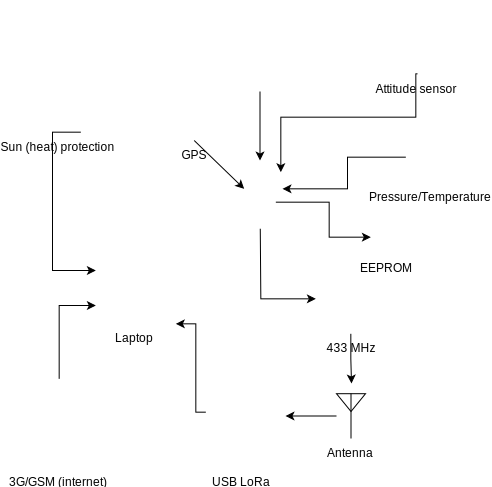
\includegraphics[scale=0.65]{GCS.svg}
\centering
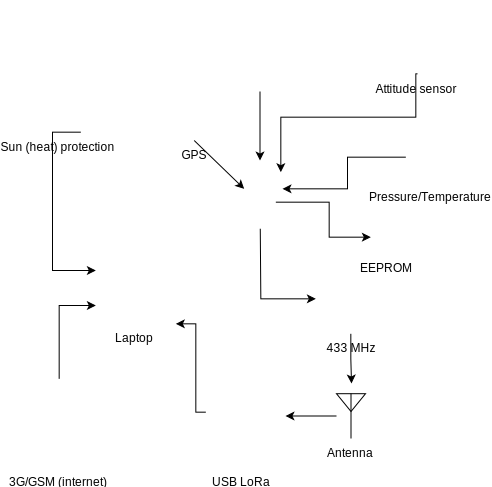
\includegraphics[scale=0.8]{GCS.png}
\caption{Ground Control Station diagram}
\label{fig:gcs}
\end{figure}

\subsection{Ground Station}
Figure \ref{fig:gcs} shows a diagram of the GCS.
\subsection{Components and Connections}
As shown in Figure \ref{fig:gcs}, the GCS will consist of:
\begin{itemize}
	\item Laptop for realtime/post processing
    \item Umbrella to cool laptop down in hot environment
    \item 3G/GSM connectivity for internet
    \item USB LoRa to receive data from CanSat
    \item Optionally a spare battery in case of bad weather conditions
\end{itemize}
\subsection{Requirements}

\begin{figure}
\centering
\includegraphics[scale=0.4]{anim_matlab.png}
\caption{Animated Matlab graph example}
\label{fig:matanim}
\end{figure}

\begin{figure}
\centering
\includegraphics[scale=0.28]{amCharts.png}
\caption{amCharts example}
\label{fig:amcharts}
\end{figure}

The GCS must be able to do real-time processing on the telemetry data. This includes real-time plotting. Matlab does have animated plotting functionality (see Figure \ref{fig:matanim}). However, amCharts (see Figure \ref{fig:amcharts}) has arguably one of the best real-time plotting engines.\\

The GCS must also be able to do post-processing on the attitude data. For example, flight trajectory

\begin{figure}
\centering
\includegraphics[scale=0.6]{flight_path.png}
\caption{CanSat flight trajectory\\
Reproduced from \cite{gopher}}
\label{fig:flight_path}
\end{figure}


\newpage

\section{CanSat Integration and Test}
\subsection{Subsystem Level Testing Plans}
\subsection{Integrated Level Functional Testing Plans}
\subsection{Environmental Testing Plans}


\newpage

\section{Mission Operations}
\subsection{Preliminary Launch Day}
\subsection{Integrated Level Functional Testing Plans}
\subsection{Environmental Testing Plans}
\subsection{Possible Risks}
The risk matrix has been constructed.
\begin{figure}[H]
\centering
\includegraphics[scale =0.4]{risk.JPG}
\label{fig:risk}
\caption{Risk Matrix}
\end{figure}

\newpage

\section{Requirements Compliance}

\section{Conclusion}




\subsection{How to add Tables}

Use the table and tabular commands for basic tables --- see Table~\ref{tab:widgets}, for example. 

\begin{table}
\centering
\begin{tabular}{l|r}
Item & Quantity \\\hline
Widgets & 42 \\
Gadgets & 13
\end{tabular}
\caption{\label{tab:widgets}An example table.}
\end{table}

\subsection{How to write Mathematics}

\LaTeX{} is great at typesetting mathematics. Let $X_1, X_2, \ldots, X_n$ be a sequence of independent and identically distributed random variables with $\text{E}[X_i] = \mu$ and $\text{Var}[X_i] = \sigma^2 < \infty$, and let
\[S_n = \frac{X_1 + X_2 + \cdots + X_n}{n}
      = \frac{1}{n}\sum_{i}^{n} X_i\]
denote their mean. Then as $n$ approaches infinity, the random variables $\sqrt{n}(S_n - \mu)$ converge in distribution to a normal $\mathcal{N}(0, \sigma^2)$.


\subsection{How to create Sections and Subsections}

Use section and subsections to organize your document. Simply use the section and subsection buttons in the toolbar to create them, and we'll handle all the formatting and numbering automatically.

\subsection{How to add Lists}

You can make lists with automatic numbering \dots

\begin{enumerate}
\item Like this,
\item and like this.
\end{enumerate}
\dots or bullet points \dots
\begin{itemize}
\item Like this,
\item and like this.
\end{itemize}

\subsection{How to add Citations and a References List}

You can upload a \verb|.bib| file containing your BibTeX entries, created with JabRef; or import your \href{https://www.overleaf.com/blog/184}{Mendeley}, CiteULike or Zotero library as a \verb|.bib| file. You can then cite entries from it, like this: \cite{greenwade93}. Just remember to specify a bibliography style, as well as the filename of the \verb|.bib|.

You can find a \href{https://www.overleaf.com/help/97-how-to-include-a-bibliography-using-bibtex}{video tutorial here} to learn more about BibTeX.

We hope you find Overleaf useful, and please let us know if you have any feedback using the help menu above --- or use the contact form at \url{https://www.overleaf.com/contact}!

\newpage
\bibliographystyle{plain}
% \bibliographystyle{alpha}
\bibliography{references}

\end{document}